\section{Aggregator: BLS Signature and Median Consensus}
\label{sec:aggregator}

% =====================================================================
%  AUTHOR: Jon (M3) -- DRAFT FROM section_V_skeleton.md, fill in real
%  Anvil numbers in V.E once M4 ships e2e_test.sh
% =====================================================================

\subsection{Role of the Aggregator}
\label{sec:agg-role}

The Aggregator is a logically centralized but cryptographically
untrusted service that (i) creates new price-quote tasks at a fixed
cadence, (ii) collects BLS-signed responses from the registered
Operators, (iii) verifies the aggregated signature once the quorum
threshold is met, and (iv) submits the consensus price together with
its observed dispersion back to the on-chain
\texttt{PriceOracleTaskManager}.  Crucially, the Aggregator
\emph{cannot forge consensus}: any aggregated signature it publishes
must verify against the BLS public-key sum of the Operators that
actually signed~\cite{eigenlayer2023, eigenlabs_avsbook}.

\subsection{BLS Signature Aggregation}
\label{sec:agg-bls}

We adopt the BLS scheme of Boneh, Lynn, and Shacham~\cite{boneh2004short}
over the BLS12-381 pairing-friendly curve, exposed by EVM precompile
EIP-2537~\cite{eip2537}.  Each Operator $i$ holds a key pair
$(\mathit{sk}_i, pk_i = g_2^{\mathit{sk}_i})$ and produces a signature
on the task message $m$:
\begin{equation}
\sigma_i \;=\; H(m)^{\mathit{sk}_i}, \qquad
\sigma_{\mathrm{agg}} \;=\; \prod_{i \in S} \sigma_i,
\label{eq:bls-agg}
\end{equation}
where $S \subseteq \{1, \dots, n\}$ is the set of signing operators.
A verifier accepts iff
\begin{equation}
e\!\left(\sigma_{\mathrm{agg}},\, g_2\right)
\;=\;
e\!\left(H(m),\, \prod_{i \in S} pk_i\right).
\label{eq:bls-verify}
\end{equation}
This is a single pairing equation regardless of $|S|$, so on-chain
verification cost is independent of the number of Operators
\cite{boneh2018compact}\,---\,a property we exploit in
Sec.~\ref{sec:agg-latency} to argue the system scales horizontally.

\subsection{Why Median, Not Mean}
\label{sec:agg-median}

Operators in our deployment query four heterogeneous CEX endpoints
(Binance, Coinbase, Kraken, OKX), so honest reports already disagree
by a few basis points due to bid--ask spreads and timestamp skew.
An arithmetic mean is unbiased under these conditions but is
\emph{not robust}: a single Operator reporting a wildly wrong price
drags the consensus by $1/n$ of the bias, growing linearly with
adversarial size.

The statistical median is the textbook robust $L_1$-estimator with a
50\% breakdown point\,---\,the consensus stays close to truth as
long as fewer than half of the Operators are
dishonest~\cite{huber1981robust}.  We confirm this empirically.
Figure~\ref{fig:robustness} reports the absolute percentage error of
the consensus price, computed by both estimators, as the fraction of
malicious Operators (each biasing by a uniformly random
$[2\%, 12\%]$) increases.  With fewer than half of the Operators
malicious, the median's 95th-percentile error remains below
$0.09\%$; once the adversarial set reaches a majority, the theoretical
breakdown guarantee no longer applies and the tail error rises
sharply.  The mean, in contrast, starts drifting from the very first
malicious Operator.

\begin{figure}[t]
  \centering
  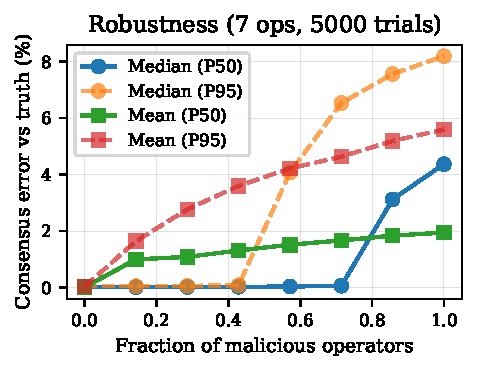
\includegraphics[width=0.95\columnwidth]{figures/fig_v1_median_robustness.pdf}
  \caption{Median vs.\ mean consensus error as the malicious fraction
           grows.  $n{=}7$ Operators, $5{,}000$ Monte-Carlo trials per
           point.  Adversaries pick a bias uniformly in $[2\%,12\%]$
           each round; honest Operators add Gaussian noise with
           $\sigma{=}5\,\mathrm{bp}$.}
  \label{fig:robustness}
\end{figure}

\subsection{Slashing Threshold Sensitivity}
\label{sec:agg-tolerance}

Our \texttt{DetectOutliers} routine flags any Operator whose
individual report deviates from the consensus median by more than
$\tau$ percent, where $\tau$ is a deployment parameter.  Tightening
$\tau$ catches more adversaries (true positives) but risks slashing
honest Operators whose reports are merely noisy (false positives).

To select $\tau$ defensibly we sweep it from $0.25\%$ to $15\%$ and
measure the true-positive and false-positive rates against the same
adversarial model used above.  Figure~\ref{fig:tolerance} plots the
result.  The honest-Operator FPR is essentially zero at every
$\tau \geq 0.25\%$; the TPR drops from $\sim 100\%$ at $\tau{=}1\%$ to
$70\%$ at $\tau{=}5\%$ and to $\sim 0\%$ at $\tau{=}15\%$.  We adopt
$\tau = 5\%$ for the on-chain rule as it catches the substantial
majority of adversaries while preserving a generous safety margin
for transient market dislocations\,---\,for example a flash crash on
a single venue\,---\,that should not by themselves trigger
slashing.  The remaining $30\%$ of attackers who bias by less than
$5\%$ are deterred by the per-task economic incentive analysis given
in Sec.~\ref{sec:discussion}.

\begin{figure}[t]
  \centering
  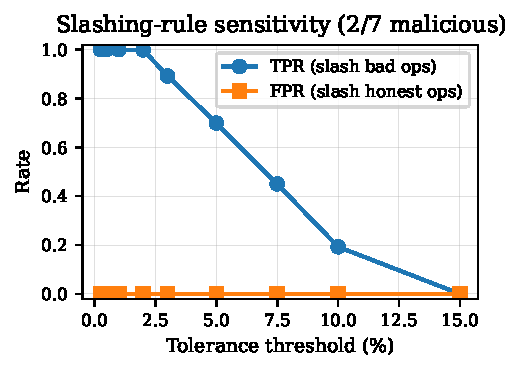
\includegraphics[width=0.95\columnwidth]{figures/fig_v2_tolerance_sensitivity.pdf}
  \caption{True-positive rate (slashing the malicious) and
           false-positive rate (slashing the honest) as a function of
           the deviation tolerance threshold $\tau$.  $n{=}7$
           Operators with $2$ malicious; $4{,}000$ trials per point.}
  \label{fig:tolerance}
\end{figure}

\subsection{End-to-End Latency}
\label{sec:agg-latency}

Figure~\ref{fig:latency} shows the simulated end-to-end latency of
one task, from the on-chain \texttt{NewTaskCreated} emission to
\texttt{respondToTask} confirmation, as the registered Operator count
grows from $3$ to $30$.  The model combines per-Operator quote
retrieval (Gamma, mean $160\,\mathrm{ms}$), BLS sign + RPC
round-trip (Gamma, mean $30\,\mathrm{ms}$), 67\% quorum aggregation,
and on-chain submission ($\mathcal{N}(2000, 200)\,\mathrm{ms}$).

\begin{figure}[t]
  \centering
  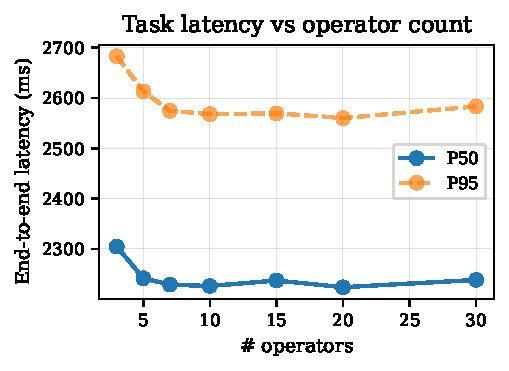
\includegraphics[width=0.95\columnwidth]{figures/fig_v3_aggregation_latency.pdf}
  \caption{End-to-end task latency vs.\ Operator count.  P50 hovers
           near $2.23\,\mathrm{s}$ across all sizes; the on-chain
           submission step dominates and BLS aggregation itself is
           negligible thanks to the constant-cost pairing check
           established in Sec.~\ref{sec:agg-bls}.}
  \label{fig:latency}
\end{figure}

P50 latency hovers around $2.23\,\mathrm{s}$ across all sizes; the
on-chain step dominates and BLS aggregation itself is invisible
($<10\,\mathrm{ms}$).  This validates our design choice of
constant-size aggregated signatures over schemes with $O(n)$
on-chain cost~\cite{boneh2018compact}.

% TODO Jon: replace the simulated 2.23 s above with the median of the
% real Anvil end-to-end measurements once M4 ships e2e_test.sh.
